% This is the TeX source for the ShabbyPages paper, using the
% LLNCS macro package for Springer Computer Science proceedings;
% Version 2.20 from 2017/10/04

\documentclass[runningheads]{llncs}
\usepackage{graphicx}
\usepackage{listings}
\usepackage{xcolor}
\lstset{basicstyle=\ttfamily,
  showstringspaces=false,
  commentstyle=\color{red},
  keywordstyle=\color{blue}
}

\begin{document}

\title{ShabbyPages, a Robust Corpus for Training Document Image Models\thanks{Supported by Sparkfish LLC.}}

\author{Alexander Groleau\inst{1} \and
  Stefan Larson\inst{2} \and
  Kok Wei Chee\inst{3}}

\authorrunning{A. Groleau et al.}
% First names are abbreviated in the running head.
% If there are more than two authors, 'et al.' is used.
%
\institute{Sparkfish, Addison TX, USA\\\and
  SkySync, Ann Arbor MI, USA\\
  \and
  \email{ck91wei@gmail.com}}
\maketitle

\begin{abstract}
This paper presents the ‘ShabbyPages’ dataset, consisting of images of documents with realistic noise properties that result from standard office operations, such as printing, scanning, and faxing through old or dirty machines, degradation of ink over time, and handwritten markings. We designed this corpus to help train and evaluate machine learning methods -- denoising, character recognition, and so on -- with text documents. The dataset and scripts to reproduce it are available on GitHub. The dataset construction process is described, with attention paid to the decisions made.

\keywords{optical character recognition \and image processing \and denoising}
\end{abstract}

\section{Introduction}
Inspired by the NoisyOffice dataset~\cite{ref_noisy}, we produced ShabbyPages as a way to help train, test, and calibrate computer vision machine learning algorithms designed for working with documents. We observed several limitations to the NoisyOffice dataset (namely, lack of diversity in font sizes and noise augmentations, as well as a lack of tables, graphics, form lines, etc.). Therefore, we were particularly interested in producing a dataset more appropriate for training general denoising models, so we built and leveraged the Augraphy~\cite{ref_augraphy} document image augmentation tool to produce noise for these images. ShabbyPages consists of  clean-noisy document image pairs.

\section{Creation}
Development of the dataset occurred in stages. A team of researchers scoured the open internet for ``born-digital" documents - PDFs that were created entirely electronically, rather than scans of existing printed documents. 600 documents were collected for review, representing categories such as government press releases, corporate financial communiques, informational brochures, and many others.\\

The \textit{pdftoppm} tool was used to separate each document into its constituent pages, converting these to PNGs in the process, using GNU Parallel~\cite{ref_parallel} to distribute the job across all available cores. \texttt{parallel pdftoppm pdfs/{} pages/{} -png -r 150} took 2 minutes to process 6202 pages on a Ryzen 9 5950x.\\

From there, we used Python's \textit{cv2} library~\cite{ref_opencv} to convert each document's color channels to grayscale, and once color data was removed, we generated and applied an Augraphy pipeline. After augmenting the images, we fit each to a standard 8.5''x11'' Letter document at various DPI levels, cropping to fit where necessary. There were several possible resizing methods, but we opted to use one which simulates using a document scanner to capture an image.  Code for all of these processes is available on GitHub~\cite{ref_shabby}.

\section{ShabbyPages - An Augraphy Project}
In our investigations, we came across precious few sources of ground-truthed document images. To aid the research community in making more, we're releasing this corpus and the code we used to produce it. Training denoising models requires a large quantity of noisy data and the original clean sources, and producing this is exactly what the Augraphy library was designed to facilitate. The Augraphy team has been hard at work for several months, improving the reliability, performance, and flexibility of the project, and we're proud that it's now mature enough to produce useful datasets.\\

Building the augmentation pipeline was straightforward: we took the default Augraphy pipeline and parametrized all the augmentations within it, keeping the parameters at the top of a file for easy adjustment. Supporting scripts were written to coordinate passing images through the Augraphy pipeline and saving them to new locations, dealing with different image resolutions, and so on. It was then possible to reproduce the noising process, so a cycle of testing was conducted where we generated noised images from the pipeline, determined properties of the output we didn't want to include in a published set, and accordingly tweaked the pipeline to no longer produce those effects. We wanted the ShabbyPages corpus to serve multiple functions -- denoising, OCR, and so on -- which constrained the degree of variation tolerated in the generating code.\\

Two primary classes of modifications to this code were considered, corresponding to a change in input constants and a restriction on certain combinations of augmentations. The Augraphy API enabled a tight feedback loop here, and made it possible to iteratively narrow in on a pipeline that generated the data we wanted. Driving Augraphy is largely a matter of developing some heuristics for unacceptable data and then telling Augraphy how to avoid producing that. This enables a workflow familiar to practitioners and researchers in this field, where edits are made to a build script and the rendering job is run, in a cycle.

\section{Tuning the Pipeline}
The default augmentation pipeline has already been tuned to produce realistic output, but the parameters required some careful tweaking to achieve our goals. Even so, there wasn't a great deal of work to do here beyond fiddling with constants to add or remove sources of variation, and to reduce the probability of certain augmentations being applied together.\\

Each augmentation in the Augraphy library was designed to reliably produce a specific effect on a document image, but care must be taken to ensure the effect is appropriate to the intended use. We intend for the first release of the ShabbyPages set to see use in training denoising models, so augmentation effects that make text impossible to read were rejected. Over a period of several weeks, we adjusted inputs to bring augmentations into the Goldilocks zone: not too heavy, not too noisy, just right. As an example, here's part of the diff between pipelines built on successive days:

\noindent\fbox{\begin{minipage}{\textwidth}
{\color{red}{$\leftarrow$ bleedthrough\_intensity\_range=(0.1, 0.2)}}

{\color{blue}{$\rightarrow$   bleedthrough\_intensity\_range=(0.05, 0.15)}}\\

{\color{red}{$\leftarrow$ bleedthrough\_color\_range=(0, 224)}}

{\color{blue}{$\rightarrow$ bleedthrough\_color\_range=(32, 224)}}\\

{\color{red}{$\leftarrow$ bleedthrough\_alpha=random.uniform(0.1,0.2)}}

{\color{blue}{$\rightarrow$    bleedthrough\_alpha=random.uniform(0.05,0.1)}}
\end{minipage}}
\hspace{1cm}\\\\
\indent Augmentations in the Augraphy project are designed to produce changes mimicking those resulting from real-world processing of documents. A diverse array of effects are possible, including the incomplete deposit of ink on paper by a stamp or typeblock, staining on the page from a dirty print drum, the reduction in quality and artifacts introduced by faxing, and the shadow produced when scanning a book of a page curling away towards the binding. Several of these transformations are pairwise mutually incompatible, depending on the intended outcomes of the produced documents, and determining these pairs is a large part of the process when using Augraphy.\\

Here are a few bad pairings we found:

\begin{itemize}
\item BadPhotoCopy turns transparent clusters of noise into opaque black patches, and cannot be used with DirtyDrum.
\item Bleedthrough can produce large dark regions which Letterpress interprets as text, applying unnatural blobs of noise.
\item The combination of dithering, thresholding, and Gaussian noise makes BadPhotoCopy and Faxify destructively interact to produce unreadable text.
\end{itemize}

\begin{figure}
    \centering
    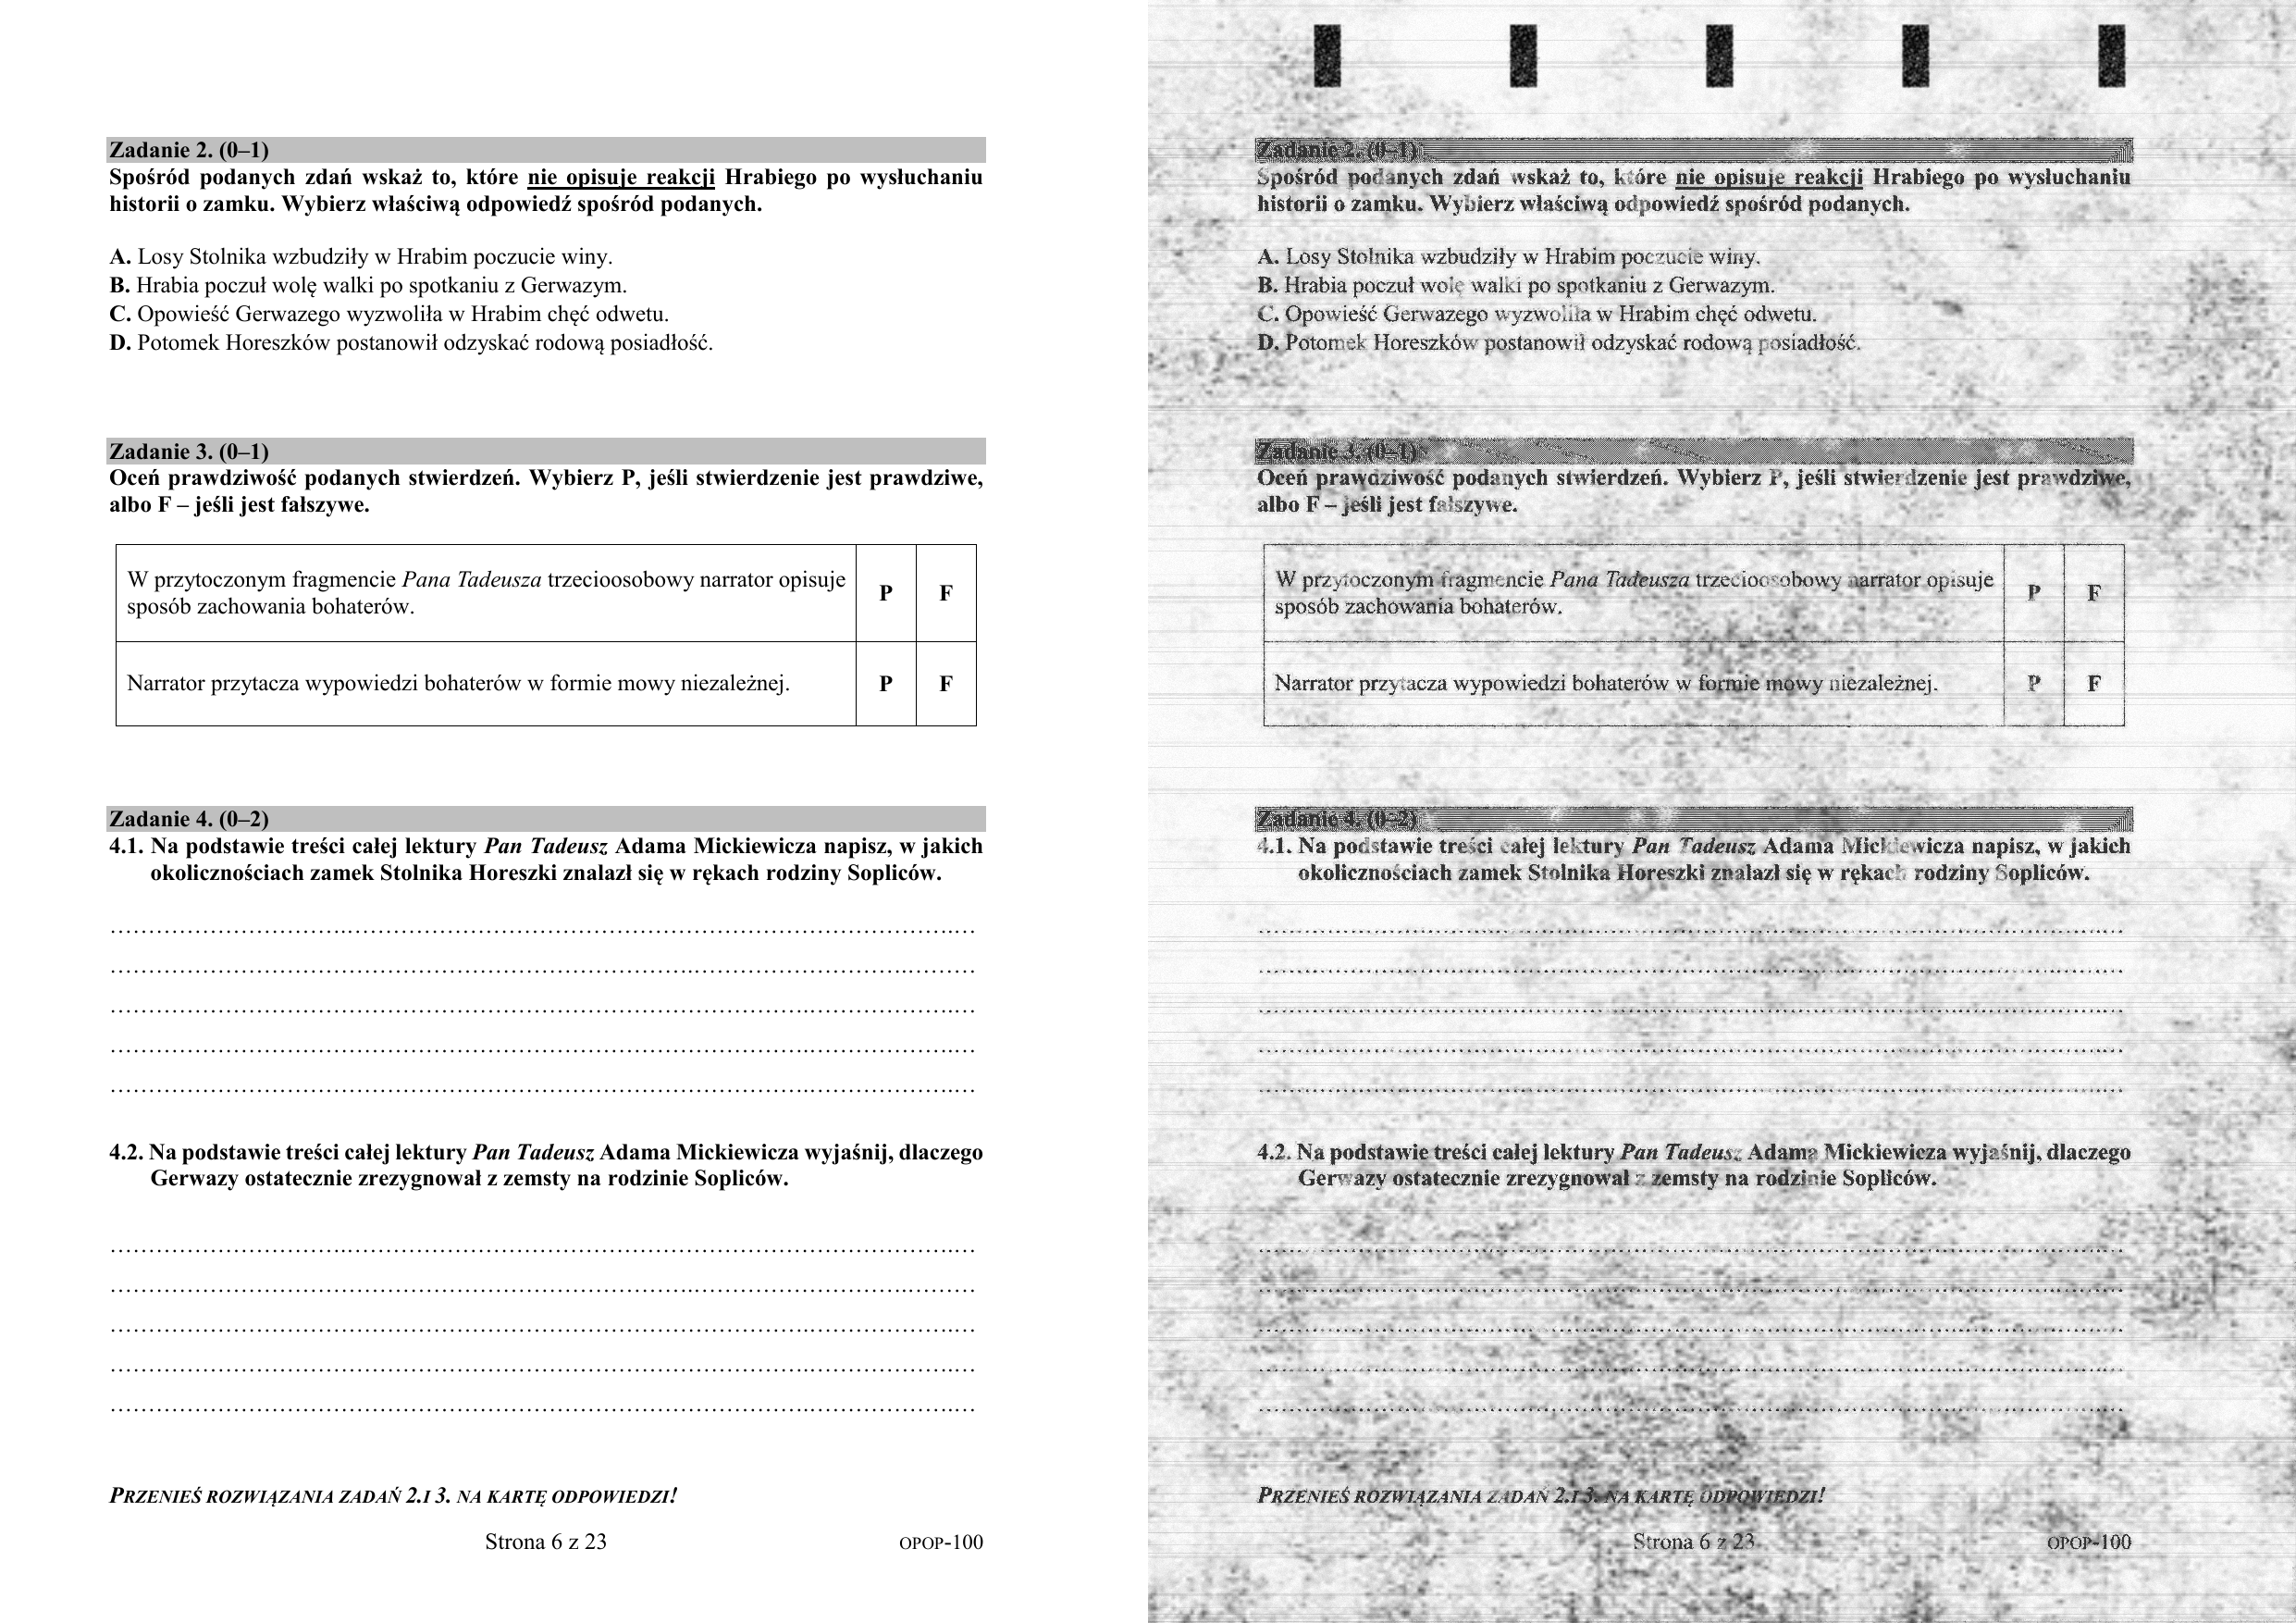
\includegraphics[width=\linewidth]{beforeafter.png}
    \caption{Example input image (left) and Augraphy-augmented output (right).}
    \label{fig:3panel}
\end{figure}

\section{Conclusion}
Compilation and production of a collection of realistically noised document images with the Augraphy tool was straightforward. The resulting dataset contains a much broader variety of noise types, font sizes, document formats, and languages than the NoisyOffice set, and the initial release is publicly available for use in denoising, recognition, and classification tasks. Scripts to facilitate dataset production with Augraphy are published on GitHub, and both these scripts and the Augraphy project itself are being actively developed.

\bibliographystyle{splncs04}

\begin{thebibliography}{5}
\bibitem{ref_noisy}
  UCI Machine Learning Repository, \url{https://archive.ics.uci.edu/ml/datasets/NoisyOffice}

\bibitem{ref_augraphy}
  Augraphy, An augmentation pipeline for rendering synthetic paper printing, faxing, scanning and copy machine processes, \url{https://github.com/sparkfish/augraphy}

\bibitem{ref_parallel}
  Tange, O. (2021, July 22). GNU Parallel 20210722 ('Blue Unity').
  Zenodo. https://doi.org/10.5281/zenodo.5123056

\bibitem{ref_opencv}
  OpenCV, \url{https://opencv.org}

\bibitem{ref_shabby}
ShabbyPages, \url{https://github.com/sparkfish/shabby-pages}
\end{thebibliography}
\end{document}
